\documentclass[11pt]{standalone}
\usepackage{amssymb}
\usepackage{amsmath}
\usepackage[no-math]{fontspec}
\usepackage{unicode-math}
\usepackage{libertinus}
\usepackage{pgf,xcolor}
\usepackage{tikz}
\usetikzlibrary{arrows.meta, backgrounds}
\usepackage{pgfplots}
\pgfplotsset{compat=newest}

\definecolor{my_darkgray}{HTML}{484949}
\definecolor{my_lightgray}{HTML}{F3F4F4}
\definecolor{my_darkblue}{HTML}{005A94}
\definecolor{my_lightblue}{HTML}{CCDEE9}
\definecolor{my_yellow}{HTML}{FFEC7F}
\definecolor{my_red}{HTML}{E60000}
\definecolor{my_orange}{HTML}{E87846}

\begin{document}
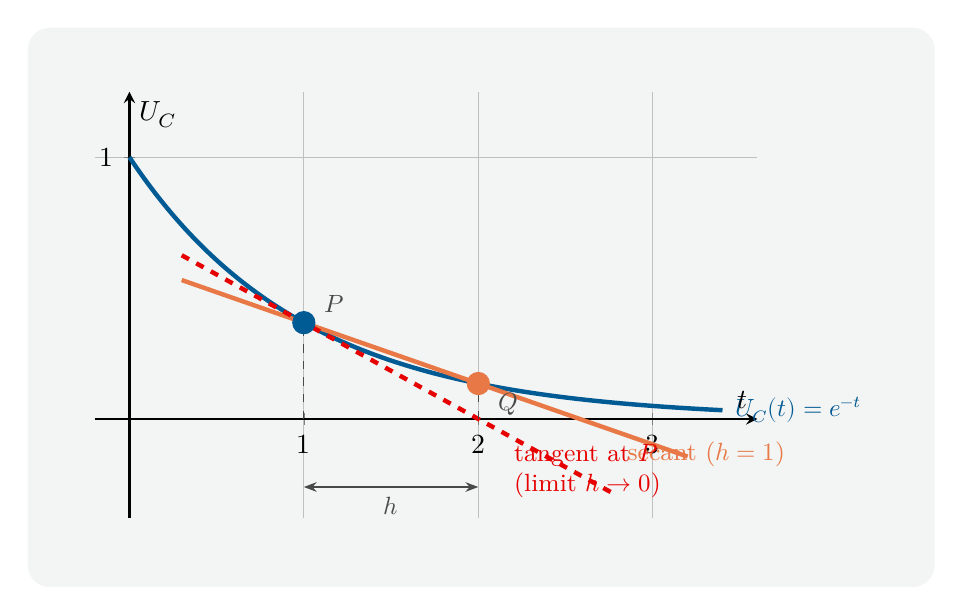
\begin{tikzpicture}[
    show background rectangle,
    background rectangle/.style={fill=my_lightgray, rounded corners=8pt},
    inner frame sep=0.8cm
]
\begin{axis}[
    axis lines=center,
    xlabel={$t$},
    ylabel={$U_C$},
    grid=both,
    %% axis equal omitted: x-range [0,3] vs y-range [0,1] would produce
    %% an unreadably flat graph at equal scaling.
    axis line style={thick},
    xmin=-0.2, xmax=3.6,
    ymin=-0.38, ymax=1.25,
    xtick={0, 1, 2, 3},
    ytick={0, 1},
    width=10cm, height=7cm,
    clip=false,
]

%% ---- Discharge curve  U_C(t) = e^{-t}  --------------------------------
\addplot[draw=my_darkblue, samples=300, ultra thick, domain=0:3.4]
    { exp(-x) };

%% Inline label at the right end of the curve
\node[anchor=west, font=\small, text=my_darkblue]
    at (axis cs:3.42, 0.033) {$U_C(t)=e^{-t}$};

%% ---- Secant through P=(1, e^{-1}) and Q=(2, e^{-2})  -----------------
%%   slope  = e^{-2} - e^{-1} = 0.13534 - 0.36788 = -0.23254
%%   through P: y = -0.23254 (x-1) + 0.36788 = -0.23254 x + 0.60042
\addplot[draw=my_orange, ultra thick, domain=0.3:3.2]
    { -0.23254*x + 0.60042 };

%% Inline label near the right end of the secant
\node[anchor=north west, font=\small, text=my_orange]
    at (axis cs:2.8, -0.05) {secant ($h=1$)};

%% ---- Tangent at P=(1, e^{-1})  ----------------------------------------
%%   slope  = -e^{-1} = -0.36788
%%   through P: y = -0.36788 (x-1) + 0.36788 = -0.36788 x + 0.73576
\addplot[draw=my_red, ultra thick, dashed, domain=0.3:2.8]
    { -0.36788*x + 0.73576 };

%% Inline label near the right end of the tangent
\node[anchor=north west, font=\small, text=my_red]
    at (axis cs:2.15, -0.06) {tangent at $P$};
\node[anchor=north west, font=\small, text=my_red]
    at (axis cs:2.15, -0.17) {(limit $h\to 0$)};

%% ---- Fixed point  P=(1, e^{-1})  --------------------------------------
\addplot[only marks, mark=*, mark size=4pt,
    mark options={draw=my_darkblue, fill=my_darkblue}]
    coordinates {(1, 0.36788)};

\node[anchor=south west, font=\small, text=my_darkgray]
    at (axis cs:1.06, 0.37) {$P$};

%% ---- Moving point  Q=(2, e^{-2})  -------------------------------------
\addplot[only marks, mark=*, mark size=4pt,
    mark options={draw=my_orange, fill=my_orange}]
    coordinates {(2, 0.13534)};

\node[anchor=north west, font=\small, text=my_darkgray]
    at (axis cs:2.06, 0.135) {$Q$};

%% ---- h annotation: double-headed arrow below the x-axis  --------------
\draw[{Stealth[scale=0.7]}-{Stealth[scale=0.7]}, thick, draw=my_darkgray]
    (axis cs:1.0, -0.26) -- (axis cs:2.0, -0.26)
    node[midway, below, font=\small, text=my_darkgray] {$h$};

%% ---- Thin vertical guides from P and Q down to the x-axis  ------------
\draw[thin, draw=my_darkgray, dashed]
    (axis cs:1, 0.0) -- (axis cs:1, 0.36788);
\draw[thin, draw=my_darkgray, dashed]
    (axis cs:2, 0.0) -- (axis cs:2, 0.13534);

\end{axis}
\end{tikzpicture}
\end{document}
